\documentclass{beamer}

\usepackage{graphicx}
\usepackage{caption}

\begin{document}
	
	\begin{frame}[plain]
		\begin{figure}
			\centering
			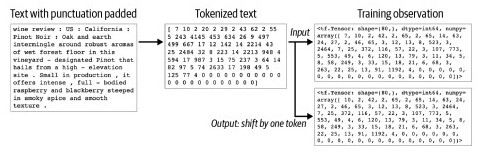
\includegraphics[width=\textwidth,height=0.85\textheight,keepaspectratio]{91.jpg}
			\caption{Data processing for the Transformer}
		\end{figure}
	\end{frame}
	
	\begin{frame}[plain]
		\begin{figure}
			\centering
			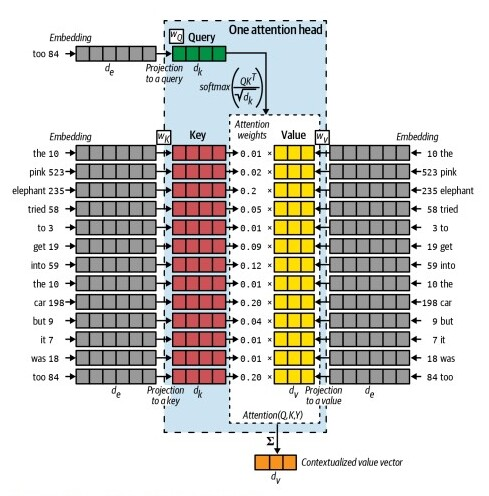
\includegraphics[width=\textwidth,height=0.85\textheight,keepaspectratio]{92.jpg}
			\caption{The mechanics of an attention head}
		\end{figure}
	\end{frame}
	
	\begin{frame}[plain]
		\begin{figure}
			\centering
			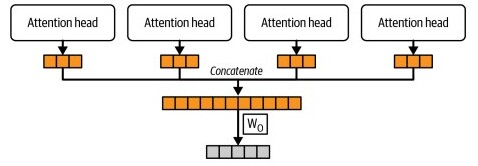
\includegraphics[width=\textwidth,height=0.85\textheight,keepaspectratio]{93.jpg}
			\caption{A multihead attention layer with four heads}
		\end{figure}
	\end{frame}
	
	\begin{frame}[plain]
		\begin{figure}
			\centering
			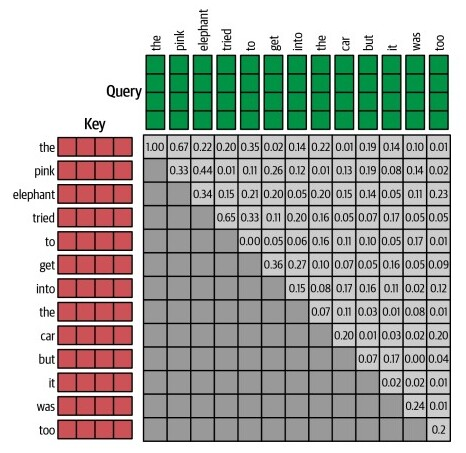
\includegraphics[width=\textwidth,height=0.78\textheight,keepaspectratio]{94.jpg}
			\caption{Matrix calculation of the attention scores for a batch of input queries, using a
				causal attention mask to hide keys that are not available to the query (because they
				come later in the sentence)}
		\end{figure}
	\end{frame}
	
	\begin{frame}[plain]
		\begin{figure}
			\centering
			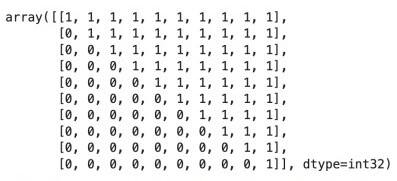
\includegraphics[width=\textwidth,height=0.8\textheight,keepaspectratio]{95.jpg}
			\caption{The causal mask as a numpy array—1 means unmasked and 0 means
				masked}
		\end{figure}
	\end{frame}
	
	\begin{frame}[plain]
		\begin{figure}
			\centering
			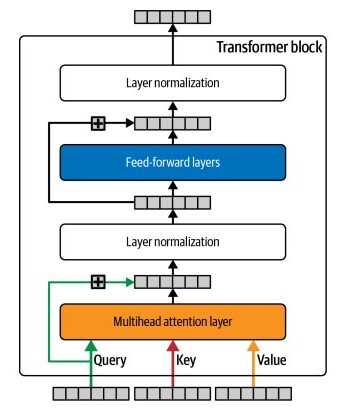
\includegraphics[width=\textwidth,height=0.85\textheight,keepaspectratio]{96.jpg}
			\caption{A Transformer block}
		\end{figure}
	\end{frame}
	
	\begin{frame}[plain]
		\begin{figure}
			\centering
			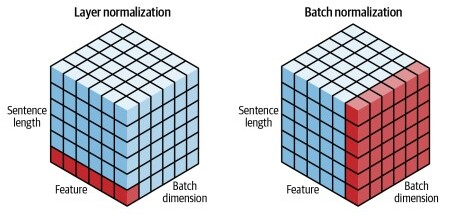
\includegraphics[width=\textwidth,height=0.85\textheight,keepaspectratio]{97.jpg}
			\caption{Layer normalization versus batch normalization—the normalization statis‐
				tics are calculated across the blue cells}
		\end{figure}
	\end{frame}
	
	\begin{frame}[plain]
		\begin{figure}
			\centering
			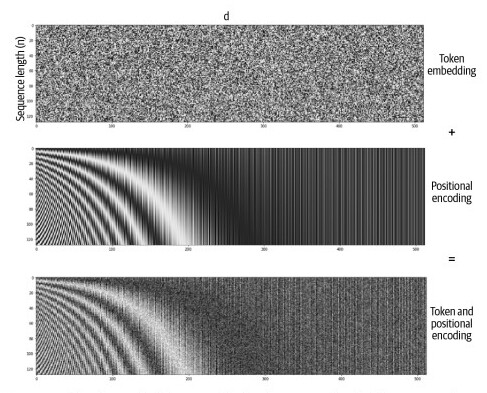
\includegraphics[width=\textwidth,height=0.85\textheight,keepaspectratio]{98.jpg}
			\caption{The token embeddings are added to the positional embeddings to give the
				token position encoding}
		\end{figure}
	\end{frame}
	
	\begin{frame}[plain]
		\begin{figure}
			\centering
			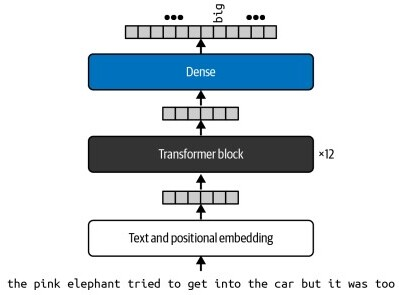
\includegraphics[width=\textwidth,height=0.85\textheight,keepaspectratio]{99.jpg}
			\caption{The simplified GPT model architecture}
		\end{figure}
	\end{frame}
	
	\begin{frame}[plain]
		\begin{figure}
			\centering
			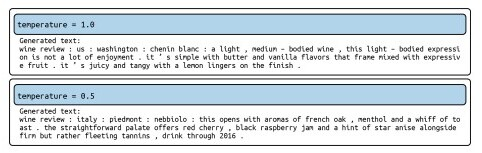
\includegraphics[width=\textwidth,height=0.85\textheight,keepaspectratio]{910.jpg}
			\caption{Generated outputs at temperature = 1.0 and temperature = 0.5.}
		\end{figure}
	\end{frame}
	
	\begin{frame}[plain]
		\begin{figure}
			\centering
			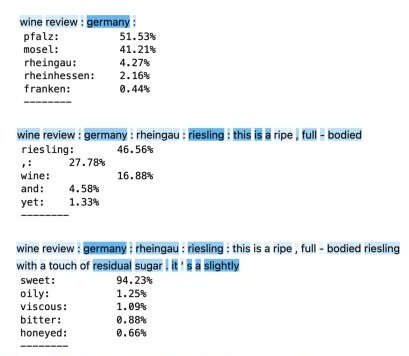
\includegraphics[width=\textwidth,height=0.85\textheight,keepaspectratio]{911.jpg}
			\caption{Distribution of word probabilities following various sequences}
		\end{figure}
	\end{frame}
	
	\begin{frame}[plain]
		\begin{figure}
			\centering
			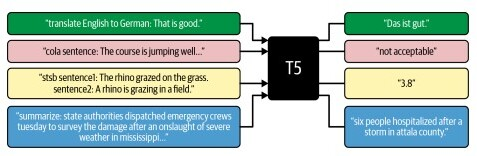
\includegraphics[width=\textwidth,height=0.85\textheight,keepaspectratio]{912.jpg}
			\caption{Examples of how T5 reframes a range of tasks into a text-to-text frame‐
				work, including translation, linguistic acceptability, sentence similarity, and document
				summarization}
		\end{figure}
	\end{frame}	
	
	\begin{frame}[plain]
		\begin{figure}
			\centering
			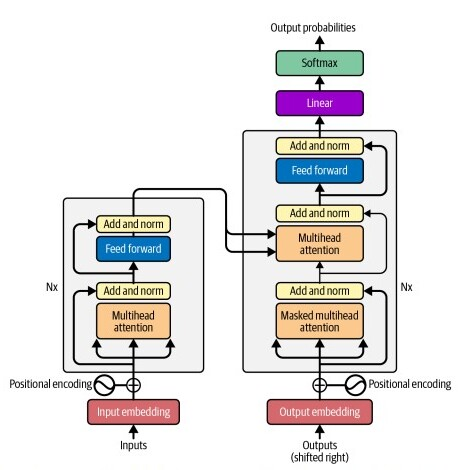
\includegraphics[width=\textwidth,height=0.85\textheight,keepaspectratio]{913.jpg}
			\caption{An encoder-decoder Transformer model: each gray box is a Transformer
				block}
		\end{figure}
	\end{frame}
	
	\begin{frame}[plain]
		\begin{figure}
			\centering
			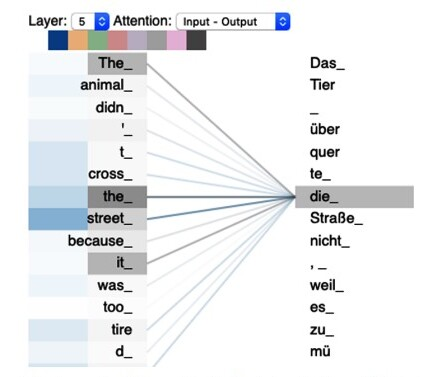
\includegraphics[width=\textwidth,height=0.7\textheight,keepaspectratio]{914.jpg}
			\caption{An example of how one attention head attends to the word “the” and
				another attends to the word “street” in order to correctly translate the word “the” to the
				German word “die” as the feminine definite article of “Straße”}
		\end{figure}
	\end{frame}
	
	\begin{frame}[plain]
		\begin{figure}
			\centering
			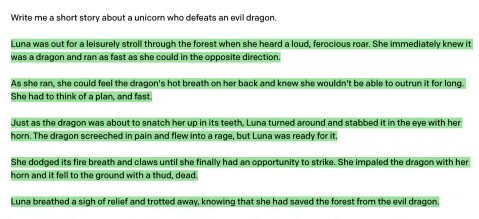
\includegraphics[width=\textwidth,height=0.85\textheight,keepaspectratio]{915.jpg}
			\caption{An example of how GPT-3 can extend a given system prompt}
		\end{figure}
	\end{frame}
	
	\begin{frame}[plain]
		\begin{figure}
			\centering
			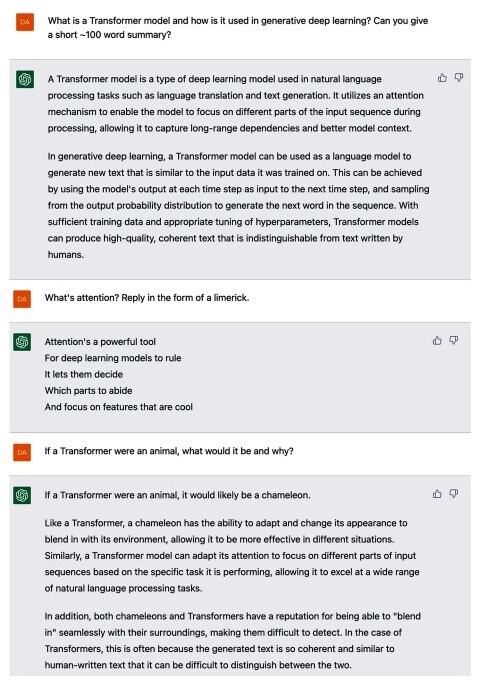
\includegraphics[width=\textwidth,height=0.85\textheight,keepaspectratio]{916.jpg}
			\caption{An example of ChatGPT answering questions about Transformers}
		\end{figure}
	\end{frame}
	
	\begin{frame}[plain]
		\begin{figure}
			\centering
			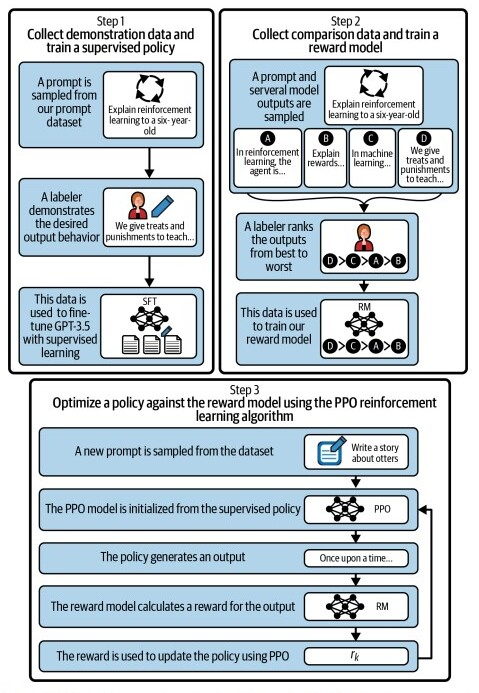
\includegraphics[width=\textwidth,height=0.85\textheight,keepaspectratio]{917.jpg}
			\caption{The reinforcement learning from human feedback fine-tuning process used
				in ChatGPT}
		\end{figure}
	\end{frame}
	
\end{document}